%==============================================================================
%  Echo In Your Words (EIYW) -- paper draft
%
%  Self-contained, compiles with a stock LaTeX install (article class + common
%  packages: booktabs, amsmath, graphicx, hyperref). No conference .sty needed --
%  swap \documentclass for acl/neurips later. Result cells are left blank ("--")
%  for future filling; search for "TODO" to find every placeholder.
%==============================================================================
\documentclass[11pt]{article}

\usepackage[utf8]{inputenc}
\usepackage[T1]{fontenc}
\usepackage{amsmath,amssymb}
\usepackage{booktabs}
\usepackage{graphicx}
\usepackage{array}
\usepackage{multirow}
\usepackage{xspace}
\usepackage[margin=1in]{geometry}
\usepackage[hidelinks]{hyperref}

% --- handy macros -------------------------------------------------------------
\newcommand{\method}{\textsc{EIYW}\xspace}      % our method
\newcommand{\lcfx}{\textsc{LCF-X}\xspace}        % the latent baseline
\newcommand{\ttt}{\textsc{T2T}\xspace}           % text-to-text baseline
\newcommand{\sharer}{\textsf{Sharer}\xspace}
\newcommand{\receiver}{\textsf{Receiver}\xspace}
\newcommand{\TODO}[1]{\textcolor{red}{[TODO: #1]}}
\usepackage{xcolor}
\newcommand{\res}{--}                             % empty result cell

\title{\textbf{Echo In Your Words}:\\
Receiver-Anchored Latent Communication Between\\
Frozen Heterogeneous Language Models}

\author{
  Jiyao Liu\\
  \texttt{\TODO{affiliation / email}}
}
\date{\today}

\begin{document}
\maketitle

\begin{abstract}
When two language models cooperate on a task, they typically communicate in
natural language: one model writes a message, the other reads it. This text
channel is lossy and rigid---it forces a continuous internal state through a
discrete vocabulary bottleneck, and what gets said is chosen without any
knowledge of what the listener actually needs. We study \emph{latent
communication}, in which a \sharer model passes information to a \receiver model
through learned continuous representations rather than text, while both base
models remain frozen. We introduce \method (\emph{Echo In Your Words}), a method
that translates the \sharer's key--value (KV) cache into a small set of
\emph{receiver-anchored soft pseudo-tokens} that are prepended to the
\receiver's input. The key idea is \emph{receiver-anchoring}: a learnable query
bank is modulated by the \receiver's own question, so \emph{what is communicated
depends on what the listener is trying to do}, not only on how the \sharer
encoded its context. A single lightweight translator module bridges arbitrary
\sharer/\receiver architectures, enabling communication between heterogeneous
model families (e.g.\ Llama~$\rightarrow$~Gemma). We evaluate on cross-context
multi-hop question answering (HotpotQA-bridge and MuSiQue), comparing against a
no-communication floor, a natural-language messaging baseline (\ttt), and a
KV-residual latent baseline (\lcfx). \TODO{one-sentence headline result once
experiments are run.}
\end{abstract}

%==============================================================================
\section{Introduction}
%==============================================================================
Multi-model and multi-agent systems increasingly rely on one model passing
information to another: a retriever summarizes for a reader, a tool-using agent
briefs a planner, a small specialist hands off to a large generalist. The
default communication channel is \emph{natural language}---model $S$ writes a
message, model $R$ reads it. This is convenient and interpretable, but it has
two structural weaknesses:
\begin{enumerate}
  \item \textbf{Discretization loss.} The \sharer holds a rich continuous state
  (its hidden activations / KV cache) but must collapse it into a discrete token
  sequence. Much of what it ``knows'' cannot be expressed faithfully, and
  decoding the message costs autoregressive steps.
  \item \textbf{Listener-blind content selection.} The \sharer writes its
  message before knowing precisely what the \receiver needs. In a cross-context
  task---where the \sharer holds one piece of evidence and the \receiver another
  ---the \sharer cannot tailor its message to the \receiver's specific
  information gap.
\end{enumerate}

\paragraph{Latent communication.} An alternative is to let the \sharer
communicate through \emph{continuous} representations that the \receiver
consumes directly, keeping both base models frozen and training only a small
bridge module. Prior work in this project (\lcfx) pools the \sharer's KV cache
into a per-layer, position-free summary and injects it as a gated KV
\emph{residual} added to \emph{every} \receiver position. This removes the
discretization bottleneck but is still \emph{listener-blind}: the summary is a
function of the \sharer's context alone.

\paragraph{Our approach: receiver-anchoring.} We propose \method, which makes
the communicated content a function of \emph{both} the \sharer's context and the
\receiver's task. \method translates the \sharer's KV cache into $K$ soft
pseudo-tokens \emph{in the \receiver's embedding space} and prepends them to the
\receiver's input, so the \receiver attends to them natively. Crucially, the
translator's query bank is modulated (FiLM-style) by an \emph{anchor}---a pooled
embedding of the \receiver's own question---so the soft tokens encode
``\emph{what the \sharer knows that is relevant to what the \receiver is
asking}.'' A single translator bridges arbitrary
$(\text{layers},\text{heads},\text{head\_dim})\rightarrow\text{hidden}$, so
heterogeneous model pairs work unchanged.

\paragraph{Contributions.}
\begin{itemize}
  \item We introduce \emph{receiver-anchored} latent communication: the
  communicated representation is conditioned on the \receiver's task, not only
  the \sharer's encoding (Section~\ref{sec:method}).
  \item We realize it as \method, a soft-pseudo-token translator that prepends
  $K$ learned tokens to a frozen \receiver and bridges heterogeneous
  \sharer/\receiver architectures with one module.
  \item We provide a controlled evaluation harness comparing a no-communication
  floor, natural-language messaging (\ttt), KV-residual latent fusion (\lcfx),
  and \method on cross-context multi-hop QA (Section~\ref{sec:experiments}).
\end{itemize}

%==============================================================================
\section{Related Work}
%==============================================================================
\paragraph{Natural-language model-to-model communication (\ttt).} The simplest
cooperation protocol has the \sharer emit a text message that the \receiver
conditions on. We include this as the \ttt baseline. It is interpretable but
incurs discretization loss and decoding latency, and selects content without
listener conditioning.

\paragraph{Latent / KV-cache fusion (\lcfx).} \lcfx is the latent baseline this
work builds on. It pools the \sharer KV cache into a single position-free
summary per layer and broadcasts it as a gated KV residual added to every
\receiver position, injected \emph{after} a \texttt{no\_grad} prompt prefill.
Because the residual is added post-prefill, only the short answer span carries
gradient during training, making \lcfx memory-light. \method differs in three
ways: (i) it produces soft tokens in \emph{embedding} space rather than a KV
residual; (ii) the tokens are \emph{prepended} so the \receiver attends to them
natively, rather than broadcast to all positions; and (iii) the content is
\emph{receiver-anchored}.

\paragraph{Soft prompts and prefix tuning.} Prepending learned continuous
vectors to a frozen model is the mechanism behind prompt/prefix
tuning. \method can be read as a \emph{data-dependent, cross-model} prefix: the
prepended vectors are not free parameters but are \emph{computed} from the
\sharer's KV cache and the \receiver's question by a trained translator.

\paragraph{Prompt / context compression.} Methods that compress long contexts
into a few soft tokens for a single model are related, but \method is
cross-model (the compressor reads model $S$'s cache and the consumer is a
different frozen model $R$) and \emph{receiver-anchored}.

%==============================================================================
\section{Method}\label{sec:method}
%==============================================================================
\subsection{Problem setup}
We consider a \emph{cross-context} question-answering setting. For a question
$q$, the evidence is split between two frozen models: the \sharer $S$ holds
context $c_S$ and the \receiver $R$ holds context $c_R$; neither context alone
suffices to answer $q$. $R$ must produce the answer $a$, and may receive
information from $S$ only through the communication channel under study. Both $S$
and $R$ are frozen; only a small bridge module is trained.

\subsection{Sharer encoding}
The \sharer encodes its own context and the question into a KV cache,
\[
  \texttt{summary} \;=\; \{(K^{(\ell)}, V^{(\ell)})\}_{\ell=1}^{L_S},
  \qquad K^{(\ell)},V^{(\ell)}\in\mathbb{R}^{B\times H_S\times N_S\times D_S},
\]
using the prompt template \texttt{build\_sharer\_encode\_text} (the \sharer's
context plus $q$). This forward is run under \texttt{no\_grad}: the cache is a
detached input to the translator.

\subsection{The translator}\label{sec:translator}
The translator $T_\theta$ maps the \sharer cache and a \receiver anchor to $K$
soft tokens in the \receiver's embedding space, $\mathbb{R}^{B\times K\times
H_R}$. It has three stages.

\paragraph{Stage 1: within-span pooling (keeps \sharer geometry).} The $N_S$ real
\sharer tokens of each layer are flattened to joint key/value features of
dimension $2H_SD_S$, split into $P$ spans, and pooled \emph{within} each span by
a shared learned query (a single-query attention), giving $L_S{\cdot}P$ span
tokens. This reduces sequence length while preserving the per-layer \sharer
structure.

\paragraph{Stage 2: receiver-anchored cross-attention (the novelty).} A learnable
query bank $Q_{\text{base}}\in\mathbb{R}^{K\times d}$ is modulated by the
\receiver anchor $\mathbf{u}\in\mathbb{R}^{H_R}$ (the mean-pooled embedding of
the \receiver's question prompt) in a FiLM-style additive shift,
\[
  Q \;=\; Q_{\text{base}} + W_a\,\mathbf{u},
\]
so the queries---hence \emph{what is read out of the \sharer cache}---depend on
the \receiver's task. The $K$ queries cross-attend over the $L_S{\cdot}P$ span
tokens; the value projection emits $H_R$-dimensional features, and an output
projection produces the $K$ soft tokens. This cross-attention is what bridges
arbitrary $(H_S, D_S, L_S)$ to $H_R$, so heterogeneous pairs need no special
casing.

\paragraph{Output projection and initialization.} The output projection maps into
the \receiver embedding space. A \emph{gentle} small-scale initialization
(weights $\sim\mathcal{N}(0,10^{-3})$) starts the soft tokens near---but not
exactly at---zero. Exact-zero soft embeddings are a numerical degeneracy that
makes the frozen \receiver's backward pass non-finite ($0\cdot\infty$); the
gentle init is a near-minimal, gradient-safe perturbation of the \receiver.

\subsection{Receiver decoding}
The soft tokens are prepended to the \receiver's input embeddings,
\[
  \texttt{inputs\_embeds} \;=\; [\, \underbrace{s_1,\dots,s_K}_{\text{soft}} \,;\;
  \mathrm{embed}(\text{prompt}) \,],
\]
and the \receiver decodes greedily as usual. With no soft tokens this reduces
\emph{exactly} to ordinary greedy decoding (the \receiver answering from its own
context alone), giving a clean no-communication floor.

\subsection{Training objective}
Only $T_\theta$ is trained; $S$ and $R$ are frozen. We minimize the
teacher-forced next-token cross-entropy on the gold answer tokens, with the
soft tokens prepended:
\[
  \mathcal{L}(\theta) \;=\;
  -\sum_{t} \log p_R\!\big(a_t \mid [\,T_\theta(c_S,q),\, \text{prompt},\, a_{<t}\,]\big).
\]
Because the soft tokens lead the sequence, \emph{every} prompt and answer
activation depends on them, so the \receiver forward is grad-enabled end-to-end
(unlike \lcfx, whose prefill is \texttt{no\_grad}). This is more memory-intensive;
we enable gradient checkpointing on the frozen \receiver to trade compute for
memory. The training batch is \emph{right-padded} (never left-padded): left
padding would route fully-masked leading positions through a grad-enabled
softmax over $-\infty$, producing NaNs that corrupt the shared gradient.

\subsection{Heterogeneous bridging}
A single translator spans arbitrary
$(\text{sharer\_layers}, \text{sharer\_kv\_heads}, \text{sharer\_head\_dim})
\rightarrow \text{receiver\_hidden}$. Checkpoints are stamped with the
\sharer/\receiver names and architecture, and loading hard-errors on a mismatch
(overridable), so a translator is only ever used with the pair it was trained
for.

% ----- workflow figure -------------------------------------------------------
\begin{figure}[t]
  \centering
  % The repo ships methods/eiyw/eiyw_workflow.svg; convert to PDF/PNG for LaTeX:
  %   inkscape eiyw_workflow.svg --export-type=pdf -o eiyw_workflow.pdf
  % 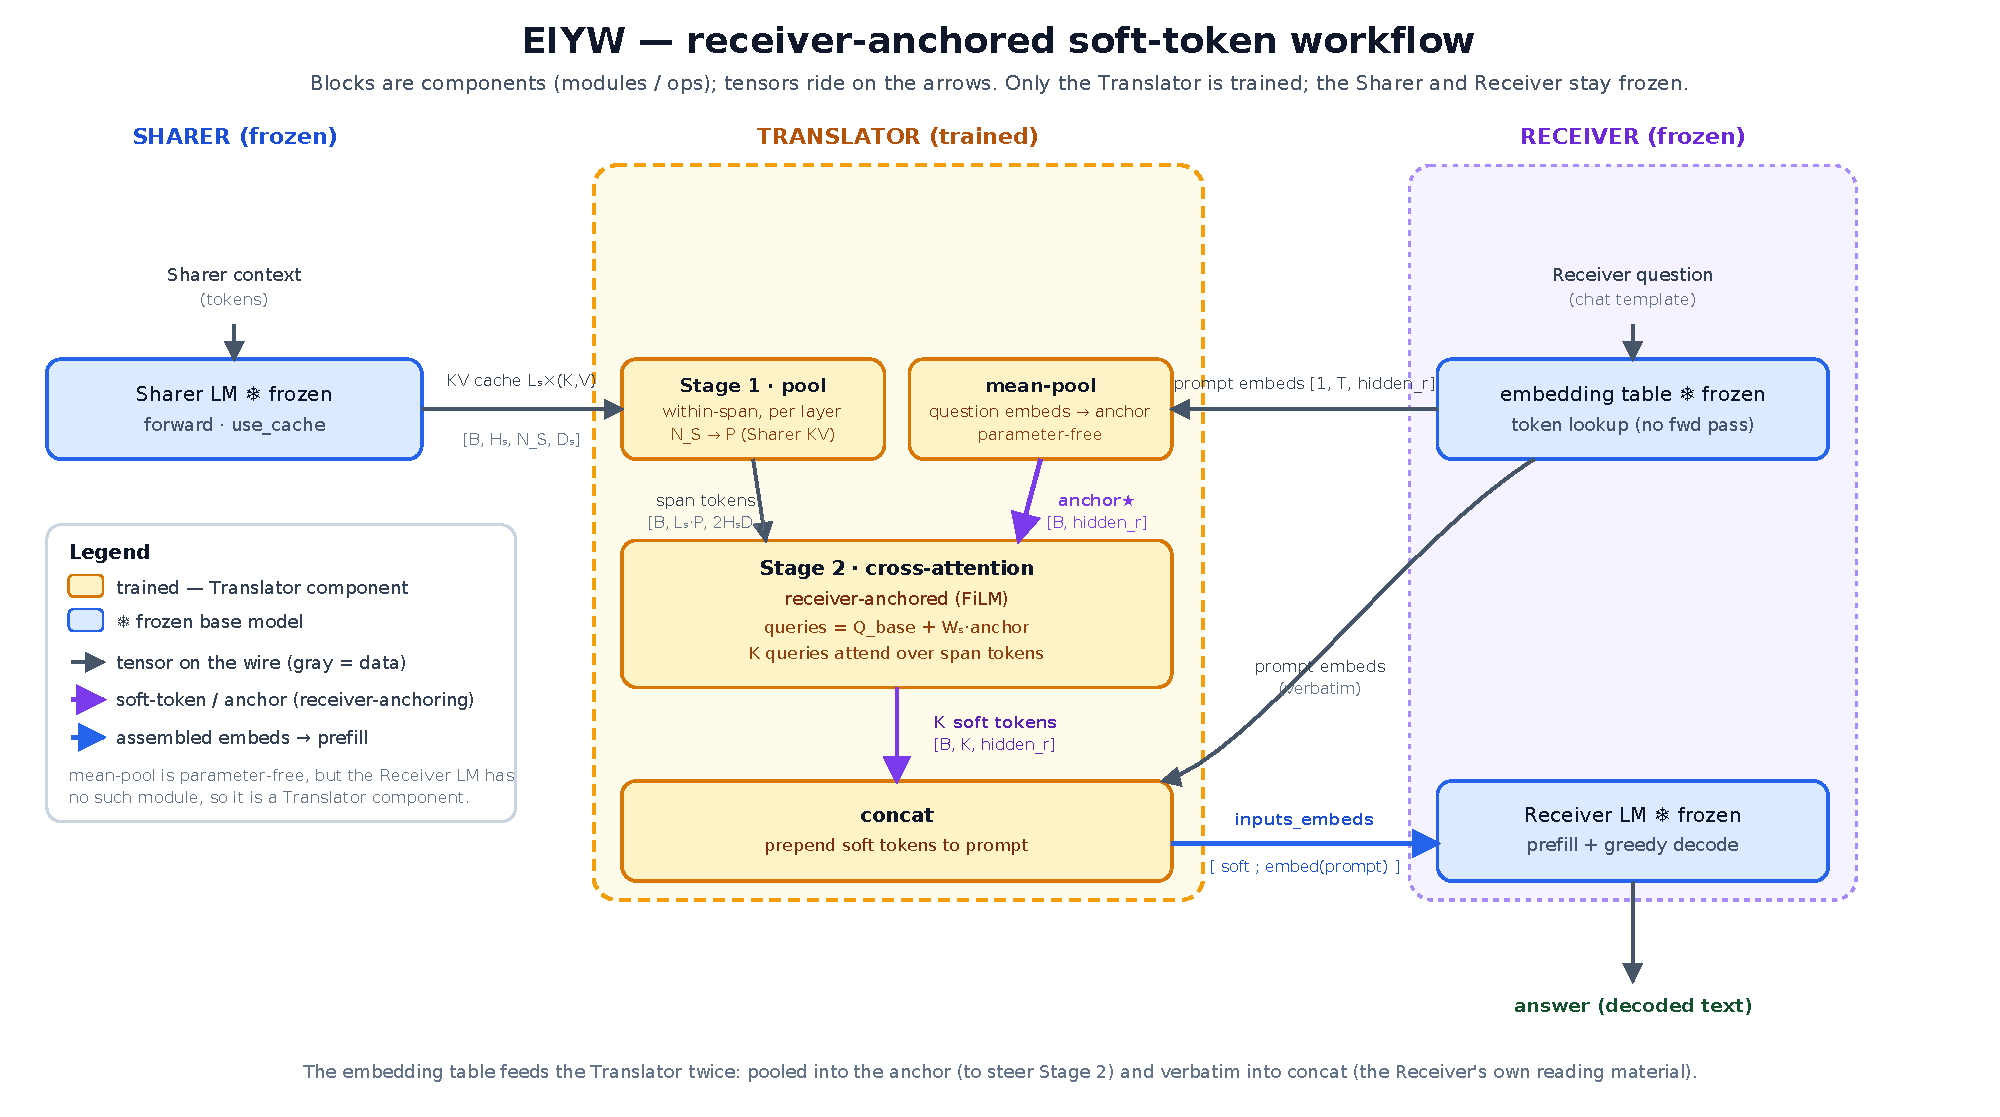
\includegraphics[width=0.9\linewidth]{eiyw_workflow.pdf}
  \fbox{\parbox{0.9\linewidth}{\centering\vspace{3em}
    \TODO{Figure: \sharer KV cache $\rightarrow$ within-span pooling $\rightarrow$
    receiver-anchored cross-attention (query bank $+$ anchor) $\rightarrow$ $K$
    soft tokens prepended to frozen \receiver. Source:
    \texttt{methods/eiyw/eiyw\_workflow.svg}.}
    \vspace{3em}}}
  \caption{The \method pipeline. Both base models are frozen; only the
  translator (shaded) is trained.}
  \label{fig:pipeline}
\end{figure}

%==============================================================================
\section{Experimental Setup}\label{sec:experiments}
%==============================================================================
\subsection{Models}
We treat the \sharer and \receiver as two independent, potentially
heterogeneous models. Table~\ref{tab:models} lists the models used; we evaluate
both a near-homogeneous Qwen pair and a cross-family (Llama~$\rightarrow$~Gemma)
pair. Gated checkpoints are accessed via ungated \texttt{unsloth/*} mirrors with
identical architectures.

\begin{table}[h]
  \centering
  \caption{Models used as \sharer and/or \receiver. \TODO{verify parameter
  counts and layer/head dims from each model config.}}
  \label{tab:models}
  \begin{tabular}{lcccc}
    \toprule
    Model & Family & Params & Layers & Hidden \\
    \midrule
    \texttt{Qwen/Qwen2.5-0.5B-Instruct} & Qwen2.5 & 0.5B & \res & \res \\
    \texttt{Qwen/Qwen3-0.6B}            & Qwen3   & 0.6B & \res & \res \\
    \texttt{Qwen/Qwen3-4B}              & Qwen3   & 4B   & \res & \res \\
    \texttt{unsloth/Llama-3.2-1B-Instruct} & Llama 3.2 & 1B & \res & \res \\
    \texttt{unsloth/gemma-3-1b-it}      & Gemma 3 & 1B   & \res & \res \\
    \bottomrule
  \end{tabular}
\end{table}

\begin{table}[h]
  \centering
  \caption{\sharer/\receiver pairs evaluated.}
  \label{tab:pairs}
  \begin{tabular}{lll}
    \toprule
    Pair & \sharer & \receiver \\
    \midrule
    Homogeneous (Qwen)   & \texttt{Qwen2.5-0.5B-Instruct} & \texttt{Qwen3-0.6B} \\
    Heterogeneous (cross-family) & \texttt{Llama-3.2-1B-Instruct} & \texttt{gemma-3-1b-it} \\
    \bottomrule
  \end{tabular}
\end{table}

\subsection{Datasets}
We use two multi-hop QA datasets, restructured into the cross-context setting:
the evidence needed to answer is split so that the \sharer holds one hop's
supporting context and the \receiver holds the other. The \receiver therefore
cannot answer without information from the \sharer.

\begin{table}[h]
  \centering
  \caption{Datasets. Scoring is free-form (Exact Match / token-level F1).
  \TODO{fill counts from \texttt{data/tasks/*.jsonl}.}}
  \label{tab:datasets}
  \begin{tabular}{llccc}
    \toprule
    Dataset & Task & \#Train & \#Val & Metric \\
    \midrule
    HotpotQA-bridge & 2-hop bridge QA (cross-context) & \res & \res & EM / F1 \\
    MuSiQue         & 2--4-hop compositional QA (cross-context) & \res & \res & EM / F1 \\
    \bottomrule
  \end{tabular}
\end{table}

\subsection{Baselines}
\begin{itemize}
  \item \textbf{Receiver-only (floor).} $R$ answers from $c_R$ alone, no
  communication. (\method with no soft tokens reduces to this exactly.)
  \item \textbf{Full-context single model (oracle ceiling).} One model answers
  from $c_S\cup c_R$ given as text---an upper bound on what perfect
  communication could achieve.
  \item \textbf{\ttt (natural-language message).} $S$ writes a text message from
  $c_S$ and $q$; $R$ answers from $c_R$ plus the message.
  \item \textbf{\lcfx (KV-residual latent fusion).} $S$'s cache is pooled and
  injected as a gated KV residual into $R$.
  \item \textbf{\method (ours).} Receiver-anchored soft pseudo-tokens prepended
  to $R$.
\end{itemize}

\subsection{Training and inference configuration}
Table~\ref{tab:hparams} lists the default translator-training recipe (shared
with the \lcfx recipe where applicable). Only the translator is trained;
gradient checkpointing is enabled on the frozen \receiver.

\begin{table}[h]
  \centering
  \caption{Default training / inference hyperparameters.}
  \label{tab:hparams}
  \begin{tabular}{ll}
    \toprule
    Setting & Value \\
    \midrule
    Optimizer & AdamW \\
    Learning rate & $1\times10^{-4}$ \\
    LR schedule & linear warmup ($200$ steps) \\
    Micro-batch size & $16$ \\
    Gradient accumulation & $16$ (effective batch $256$) \\
    Gradient clipping & $1.0$ \\
    Soft tokens $K$ & $16$ \TODO{confirm default used in runs} \\
    Pooling spans $P$ & $4$ \\
    Translator bottleneck dim & $128$ \\
    Validation holdout & $2.8\%$ of train (when no explicit eval split) \\
    Receiver max new tokens & $64$ \\
    Seed & $0$ \\
    \bottomrule
  \end{tabular}
\end{table}

%==============================================================================
\section{Results}\label{sec:results}
%==============================================================================
\noindent\emph{All result cells below are placeholders (\res) to be filled once
runs complete.}

\subsection{Main results}
Table~\ref{tab:main} reports EM/F1 for every method on both datasets and both
model pairs.

\begin{table}[h]
  \centering
  \caption{Main results: Exact Match / F1 ($\uparrow$). Best non-oracle per
  column in \textbf{bold} (fill in later).}
  \label{tab:main}
  \setlength{\tabcolsep}{5pt}
  \begin{tabular}{l cc cc}
    \toprule
    & \multicolumn{2}{c}{Qwen pair} & \multicolumn{2}{c}{Llama$\rightarrow$Gemma} \\
    \cmidrule(lr){2-3}\cmidrule(lr){4-5}
    Method & HotpotQA & MuSiQue & HotpotQA & MuSiQue \\
           & {\small EM / F1} & {\small EM / F1} & {\small EM / F1} & {\small EM / F1} \\
    \midrule
    Receiver-only (floor)      & \res & \res & \res & \res \\
    Full-context (oracle)      & \res & \res & \res & \res \\
    \midrule
    \ttt (text message)        & \res & \res & \res & \res \\
    \lcfx (KV residual)        & \res & \res & \res & \res \\
    \method (ours)             & \res & \res & \res & \res \\
    \bottomrule
  \end{tabular}
\end{table}

\subsection{Ablations}
Table~\ref{tab:ablation} isolates the contributions of the main design choices,
on \TODO{pick the primary dataset/pair, e.g.\ HotpotQA, Qwen pair}.

\begin{table}[h]
  \centering
  \caption{Ablations (EM / F1, $\uparrow$).}
  \label{tab:ablation}
  \begin{tabular}{ll cc}
    \toprule
    Group & Variant & EM & F1 \\
    \midrule
    \multirow{1}{*}{Full} & \method (default $K{=}16$, $P{=}4$, anchored) & \res & \res \\
    \midrule
    \multirow{2}{*}{Receiver-anchoring}
       & w/o anchor (query bank only)        & \res & \res \\
       & w/o anchor, content from \sharer only & \res & \res \\
    \midrule
    \multirow{3}{*}{Soft tokens $K$}
       & $K=4$   & \res & \res \\
       & $K=8$   & \res & \res \\
       & $K=32$  & \res & \res \\
    \midrule
    \multirow{2}{*}{Pooling spans $P$}
       & $P=1$ & \res & \res \\
       & $P=8$ & \res & \res \\
    \midrule
    \multirow{1}{*}{Init} & exact-zero vs.\ gentle ($10^{-3}$) & \res & \res \\
    \bottomrule
  \end{tabular}
\end{table}

\subsection{Efficiency}
Table~\ref{tab:efficiency} compares the communication cost and resource
footprint of each channel. \method trades higher \emph{training} memory
(grad-enabled prefill) for a compact, text-free message of $K$ vectors at
inference.

\begin{table}[h]
  \centering
  \caption{Efficiency. ``Message size'' is tokens (\ttt) or soft-token vectors
  (latent). Training peak memory at the default batch. \TODO{measure}.}
  \label{tab:efficiency}
  \begin{tabular}{l c c c c}
    \toprule
    Method & Message size & Latency / ex. (ms) & Train peak mem & Trainable params \\
    \midrule
    \ttt   & \res text tok & \res & n/a & n/a \\
    \lcfx  & per-layer summary & \res & \res & \res \\
    \method & $K$ vectors & \res & \res & \res \\
    \bottomrule
  \end{tabular}
\end{table}

%==============================================================================
\section{Discussion and Limitations}
%==============================================================================
\paragraph{Why receiver-anchoring should help.} In cross-context tasks the
useful content of $c_S$ depends on the \receiver's gap. Conditioning the readout
on the \receiver's question lets the translator surface exactly the bridging
fact $R$ is missing, rather than a generic summary of $c_S$. \TODO{support with
the anchor ablation once run.}

\paragraph{Limitations.}
(i) Training memory: the grad-enabled prefill makes \method roughly $2\times$
heavier than \lcfx at the same batch (mitigated by gradient checkpointing and a
smaller micro-batch with more accumulation).
(ii) Interpretability: unlike \ttt, the soft-token message is not human-readable.
(iii) Per-pair training: a translator is tied to one \sharer/\receiver pair.

%==============================================================================
\section{Conclusion}
%==============================================================================
We presented \method, a receiver-anchored latent-communication method that
translates a frozen \sharer's KV cache into question-conditioned soft
pseudo-tokens prepended to a frozen \receiver, bridging heterogeneous model
families with a single trained module. \TODO{final claim once results land.}

%==============================================================================
\appendix
\section{Reproducibility}
Entry points: \texttt{scripts/train\_eiyw.py}, \texttt{scripts/run\_eiyw.py};
baselines \texttt{scripts/run\_text\_to\_text.py}, \texttt{scripts/run\_lcfx.py},
\texttt{scripts/run\_single\_model.py}. Data preparation:
\texttt{scripts/prepare\_hotpotqa\_bridge.py},
\texttt{scripts/prepare\_musique.py}. Results are written under
\texttt{results/<method>/<dataset>/<sharer>/<receiver>/} as
\texttt{metrics.json}, \texttt{predictions.jsonl},
\texttt{predictions\_brief.tsv}, and \texttt{eval\_log.jsonl}.

\end{document}
